% !TEX encoding = IsoLatin
\documentclass{report}

%description: Rapport FICHE AUTOM AVANCEE
%%%%%%%%%%%%%%%%%%%%%%%%%%

%Insertion de packages
\usepackage[french]{babel} % pour dire que le texte est en fran?cais
\usepackage[latin1]{inputenc}
\usepackage[T1]{fontenc} % pour les font postscript
\usepackage{a4} % pour la taille
\usepackage{graphicx}
\usepackage{color}
\usepackage{listings}
\usepackage{multirow}
\usepackage{pdflscape}
\usepackage{fix-cm}
\usepackage[cyr]{aeguill} % Police vectorielle TrueType, guillemets fran?cais
\usepackage[top=3cm, bottom=3cm, left=2.5cm, right=2.5cm]{geometry} %pour les marges
\usepackage{epsfig} % pour g�erer les images
\usepackage{amsmath, amsthm} % tr`es bon mode math�ematique
\usepackage{amsfonts,amssymb}% permet la definition des ensembles
\usepackage{float} % pour le placement des figure
\usepackage{url} % pour une gestion efficace des url
\usepackage{fancyhdr}
\usepackage{fancyvrb}
\pagestyle{fancy}
\bibliographystyle{plain} % Style bibliographique
\usepackage{array}		%package pour g?rer l'environnement tableau
\usepackage[pdftex]{hyperref} % Pour les liens vers les chapitres
\hypersetup{pdfstartview=FitV, colorlinks, linkcolor=black}
\usepackage{pgfplots}
\usepackage{amsmath}

%% pas sur que tous les packages et defines soit utilies
\usepackage{listingsutf8}
\usepackage{color}
\usepackage{textcomp}

\newcommand{\HRule}{\rule{\linewidth}{0.5mm}}

%========= PAGE DE GARDE =============
% Preambule
\makeatletter
\makeatother
%=============== Corps ===============
\begin{document}

\rhead{\footnotesize\rightmark}
\chead{}
\lhead{}
\lfoot{\footnotesize BE Commande Avanc�e - R�gulation d'une turbine � gaz}
\rfoot{\footnotesize\thepage~/~\pageref{pagefin}}
\cfoot{}
\renewcommand{\headrulewidth}{0.4pt}
\renewcommand{\footrulewidth}{0.4pt}

\thispagestyle{empty}

	% !TEX encoding = IsoLatin

\begin{titlepage}

 %----------------------------
 %Upper part of the page
\begin{flushleft}
% ---- LOGO INSA -----
%\raggedright
\includegraphics[width=4cm,height=3.8cm]{./figures/logoInsa.PNG}
%-----------
\end{flushleft}
 
\begin{center}
\vspace*{1cm}
\textsc{\large BE Commande avanc�e}\\[0.7cm]
\textsc{\huge \textbf{\underline{R�gulation d'une turbine � gaz}}}\\[0.4cm]
% Title
% Author and supervisor
\begin{minipage}{1.2\textwidth}
\begin{flushleft} \large
\emph{\textit{\underline{Auteurs}:}}\\[0.25cm]
\textsc{Martin} PETROV \hspace*{1.2cm}\textit{\small{mpetrov@etud.insa-toulouse.fr}}\\
\textsc{Julien} MAFFRE \hspace*{1.2cm}\textit{\small{maffre@etud.insa-toulouse.fr}}\\
\end{flushleft}
\end{minipage}
\\[0.4cm]
\begin{minipage}{1.2\textwidth}
\begin{flushleft} \large
\emph{\textit{\underline{Enseignants}:}}\\[0.25cm]
\textsc{Charles} POUSSOT VASSAL \hspace*{1.2cm}\small{\textit{contact : charles.poussot-vassal@onera.fr}}\\
\textsc{todo} TODO \hspace*{1.2cm}\small{\textit{contact : todo@laas.fr}}\\
\end{flushleft}
\end{minipage}
\\[0.2cm]

\begin{center}
\vspace{1cm}
	\large INSA Toulouse - 5 SEC-Automatique Avanc�e \\
	\vspace{0.2cm}
	\today \\
	\vspace{0.2cm}
	\textit{version 1.0} \\
	\large
\end{center}
\hrule

\begin{center}
\vspace{0.5cm}
	\textbf{RESUME DE LA FICHE}
\end{center}

\begin{Verbatim}[frame=single,fontsize=\normalsize]
Ce compte-rendu explique en d�tails le bureau d'�tudes de Commande Avanc�e qui 
qui s'effectue dans le cadre de l'UF TODO. Test Julien Git.

Nous pr�sentons la mod�lisation et l'asservissement d'une turbine � gaz avec les 
justifications des choix et commandes diff�rents. On applique une d�marche industrielle 
en respectant des sp�cifications.

Dans l'annexe vous pouvez consulter le script Matlab utilis� pour ce bureau d'�tudes.
\end{Verbatim}
\end{center}
\end{titlepage}
	
	\tableofcontents
	
	
	% !TEX encoding = IsoLatin
\chapter*{Introduction}
\addcontentsline{toc}{chapter}{Introduction}

% introduction	
\paragraph{SUJET}
\paragraph{}Dans ce bureau d'�tude nous consid�rons le syst�me d'une turbine � gaz. Ce type de syst�me est choisi afin d'appliquer une d�marche industrielle de conception. 

\paragraph{ETAPES}
\paragraph{}L'objectif est de concevoir une commande pour la turbine qui va respecter un cahier des charges. Plusieurs comp�tences th�oriques sont n�cessaires pour la r�solution du probl�me pos�. Dans un premier temps, nous mod�liserons le syst�me avec un mod�le math�matique d�crivant son comportement. Ensuite, nous allons lin�ariser autour d'un point de fonctionnement et choisir les diff�rentes solutions possibles pour la strat�gie de contr�le afin de mieux satisfaire les sp�cifications. Nous expliquerons l'utilit� d'un filtre de Kalman pour mieux estimer le mod�le. Une commande par retour d'�tat et une discussion introductive aux techniques de commande robuste seront enfin pr�sent�es.

\paragraph{SUPPORT}
	         
\paragraph{}\textit{L'ensemble des sources du projet (Matlab/Simulink) est disponible � l'adresse suivante : \url{https://github.com/mape1991/BEcommandeAA}} 
	\clearpage{}
		
	% !TEX encoding = IsoLatin
% --------------------------------------------------------------------------------------------------------------------------------------------------------------------------- %
%\begin{itemize}
%\item [-] \textbf{Cr�ation} : Demand�e par un autre processus,  cr�e dans l'�tat pr�t ou suspendu.
%\item [-] \textbf{Destruction} : peut �tre fait par le processus lui-m�me, un autre processus, le noyau. La destruction provoque une lib�ration des ressources associ�es et un �v�nement.
%\item [-] \textbf{Blocage} : passage en mode bloqu� en attente d'un �v�nement externe. Peut �tre demand� par le processus lui-m�me ou par le syst�me.
%\item [-] \textbf{D�blocage} : passage en mode pr�t apr�s le mode bloqu� lorsque l'�v�nement attendu se produit.
%\item [-] \textbf{Activation} : passage en mode ex�cution d'un mode pr�t.
%\end{itemize}

  
%\begin{Verbatim}[frame=single,fontsize=\scriptsize]
%\end{Verbatim}

%\begin{figure}[h]
%	\begin{center}
%		\includegraphics[width=14.5cm,height=9cm]{.\figures\diag_etat_threads.png}
%	\end{center}
%	\caption{Diagramme des diff�rents �tats d'un thread avec les primitives}
%	\label{fig:diag_etat_threads}
%\end{figure}

%% Modele d'etat avec les matrices

%\begin{displaymath}
%\left\{ \begin{array}{l} \dot{x} \quad = \quad \left[ \begin{array}{cccc}
%0 & 1 & 0 & 1\\
%- \frac{K_s}{M_s} & - \frac{C_s}{M_s} & 0 & \frac{C_s}{M_s}\\
%0 & 0 & 0 & 1\\
%\frac{K_s}{M_u} & \frac{C_s}{M_u} & - \frac{K_t}{M_u} & - \frac{C_s}{M_u} - \frac{C_t}{M_u}
%
%\end{array}\right]  x \quad + \quad \left[ \begin{array}{cc}
%0 & 1.1972\\
%0 & - 0.0012\\
%0 & 0\\
%7.84 & - 4.05
%\end{array} \right] u\\ \\
%y \quad = \quad \left[ \begin{array}{cccc}
%1 & 0 & 0 & 0\\
%0 & \lambda & 0 & 0\\
%0 & 0 & \lambda & 0\\
%0 & 0 & 0 & \lambda\\
%0 & - \lambda & \lambda & 0
%\end{array} \right] x \quad + \quad \left[ \begin{array}{cc}
%0 & 0\\
%0 & 0\\
%0 & 0\\
%0 & 0\\
%0 & 0
%\end{array} \right] u \end{array}\right.
%\end{displaymath}\\

% --------------------------------------------------------------------------------------------------------------------------------------------------------------------------- %
\rhead{\footnotesize\rightmark}
\chapter{Mod�lisation du syst�me}

	\clearpage{}
	
	% !TEX encoding = IsoLatin
% --------------------------------------------------------------------------------------------------------------------------------------------------------------------------- %
%\begin{itemize}
%\item [-] \textbf{Cr�ation} : Demand�e par un autre processus,  cr�e dans l'�tat pr�t ou suspendu.
%\item [-] \textbf{Destruction} : peut �tre fait par le processus lui-m�me, un autre processus, le noyau. La destruction provoque une lib�ration des ressources associ�es et un �v�nement.
%\item [-] \textbf{Blocage} : passage en mode bloqu� en attente d'un �v�nement externe. Peut �tre demand� par le processus lui-m�me ou par le syst�me.
%\item [-] \textbf{D�blocage} : passage en mode pr�t apr�s le mode bloqu� lorsque l'�v�nement attendu se produit.
%\item [-] \textbf{Activation} : passage en mode ex�cution d'un mode pr�t.
%\end{itemize}

  
%\begin{Verbatim}[frame=single,fontsize=\scriptsize]
%\end{Verbatim}

%\begin{figure}[h]
%	\begin{center}
%		\includegraphics[width=14.5cm,height=9cm]{.\figures\diag_etat_threads.png}
%	\end{center}
%	\caption{Diagramme des diff�rents �tats d'un thread avec les primitives}
%	\label{fig:diag_etat_threads}
%\end{figure}

%% Modele d'etat avec les matrices

%\begin{displaymath}
%\left\{ \begin{array}{l} \dot{x} \quad = \quad \left[ \begin{array}{cccc}
%0 & 1 & 0 & 1\\
%- \frac{K_s}{M_s} & - \frac{C_s}{M_s} & 0 & \frac{C_s}{M_s}\\
%0 & 0 & 0 & 1\\
%\frac{K_s}{M_u} & \frac{C_s}{M_u} & - \frac{K_t}{M_u} & - \frac{C_s}{M_u} - \frac{C_t}{M_u}
%
%\end{array}\right]  x \quad + \quad \left[ \begin{array}{cc}
%0 & 1.1972\\
%0 & - 0.0012\\
%0 & 0\\
%7.84 & - 4.05
%\end{array} \right] u\\ \\
%y \quad = \quad \left[ \begin{array}{cccc}
%1 & 0 & 0 & 0\\
%0 & \lambda & 0 & 0\\
%0 & 0 & \lambda & 0\\
%0 & 0 & 0 & \lambda\\
%0 & - \lambda & \lambda & 0
%\end{array} \right] x \quad + \quad \left[ \begin{array}{cc}
%0 & 0\\
%0 & 0\\
%0 & 0\\
%0 & 0\\
%0 & 0
%\end{array} \right] u \end{array}\right.
%\end{displaymath}\\

% --------------------------------------------------------------------------------------------------------------------------------------------------------------------------- %
\rhead{\footnotesize\rightmark}
\chapter{Lin�arisation du mod�le}

	Le syst�me global \og turbine � gaz \fg �tant d�sormais mod�lis� � partir de tables de mesures (grandement non-lin�aires) sur le syst�me, il est d�sormais n�cessaire de lin�ariser le syst�me autour d'un point de fonctionnement. Le but est d'obtenir une fonction de transfert globale sur laquelle les techniques de contr�le connues pourront �tre appliqu�es. \\
	
	Le vecteur d'�tat $X$ que nous allons consid�rer est tel que : $X = [W_f \quad N_g \quad N_{tl}]^t$. Le syst�me comporte une entr�e de consigne $W_f$ (d�bit de carburant) et une entr�e de perturbation $C_{charge}$ (couple charge sur l'arbre de sortie). 

			\section{Calcul du point d'�quilibre}
			
			L'objectif de la lin�arisation est de fixer un point de fonctionnement $X_0 = [W_f^0\quad N_g^0\quad N_{tl}^0]^t$, $U_0 = [W_f^0 \quad C_{charge}^0]^t$ et de n'�tudier le syst�me que pour de petites variations de l'�tat autour de ce point statique. L'objectif de la r�gulation �tant de fixer $N_{tl}$ � $N_{tl}^{nom}$, on aura donc \textbf{$N_{tl}^0 = N_{tl}^{nom} = 22800 \:tr/min$}. Les autres variables d'�tat du syst�me �tant d�pendantes l'une de l'autre, il est alors n�cessaire de fixer l'une des deux pour calculer compl�tement le point d'�quilibre. $N_g$ �tant mesur�e de mani�re fiable, c'est cette derni�re que nous fixerons telle que \textbf{$N_{g}^0 = 28000 \:tr/min$}. \\
			
			D'apr�s l'�quation \ref{eq:cg}, nous avons : 
			\begin{equation}
				I_g\dot{N_g}(t) = C_g(W_f, N_g)	
			\end{equation}
			
			Comme $N_g$ est consid�r�e constante autour du point d'�quilibre, alors $\dot{N_g}(t) = 0$. Pour d�terminer $W_f^0$, il suffit alors de trouver l'abscisse $W_f$ pour laquelle le couple r�sultant $C_g$ s'annule, soit (cf Fig. \ref{fig:maillages}) : 
			\begin{equation}
				W_f^0 = arg ( min |C_g(W_f, N_g^0)| )
			\end{equation}
			
			La fonction Matlab \texttt{fminsearch} retourne alors \textbf{$W_f^0 = 259.64\:\:L/h$}. \\
			
			Le couple de charge $C_{charge}^0$ est alors d�termin� par la lecture du maillage de $C_{tl}(W_f^0, N_g^0)$ (cf Fig. \ref{fig:maillages}), soit donc \textbf{$C_{charge}^0 = 13.6025\:\:m.daN$}.
			

			\section{Lin�arisation}
			
				Le point d'�quilibre ($X_0$, $U_0$) �tant d�sormais d�termin�, les �quations dynamiques r�gissant l'�volution des �tats au cours du temps doivent �tre calcul�es. Il suffit alors d'effectuer un changement de variable de type $X(t) = \Delta X(t) + X_0$. \\
				
				On obtient alors l'�quation d'�tat dynamique du syst�me sous la forme : 
				
				\begin{equation}
				\begin{split}
				\dot{\Delta X} & = J_f\vert_{X=X_0}.\Delta X \\
							& + {\frac{\delta g}{\delta W_f^*}}\rvert_{W_f^{*0}}.\Delta W_f^* \\
							& + \frac{\delta h}{\delta C_{charge}}\rvert_{C_{charge}^0}. \Delta C_{charge} \\
							& + f(X_0) + g(W_f^{*0}) + h(C_{charge}^0)
				\end{split}
				\end{equation}
				
				Avec $J_f$, jacobienne de la matrice dynamique du syst�me non-lin�aire, telle que, d'apr�s les �quations \ref{eq:doseur}, \ref{eq:cg} et \ref{eq:ntl} : 
				
		\begin{equation}		
J_f =
 \begin{pmatrix}
  -\frac{1}{t_{dos}} & 0 & 0 \\
  \frac{1}{I_g}  \frac{\delta C_g(W_f,N_g)}{\delta W_f} & \frac{1}{I_g} \frac{\delta C_g(W_f,N_g)}{\delta N_g} & 0 \\
  \frac{1}{I{tot}} \frac{\delta C_{tl}(W_f,N_g,N_{tl})}{\delta N_g} & \frac{1}{I_{tot}} \frac{\delta C_{tl}(W_f,N_g,N_{tl})}{\delta N_g} & \frac{1}{I_{tot}} \frac{\delta C_{tl}(W_f,N_g,N_{tl})}{\delta N_{tl}}
 \end{pmatrix}
= 
 \begin{pmatrix}
    -18.5185   &      0       &  0 \\
   65.5871 &  -1.9835   &      0 \\
   17.1650  &  0.8011  & -0.5289
 \end{pmatrix}
	\end{equation}
	
	Par cons�quent, la matrice dynamique $A_{lin}$ du syst�me lin�aris� est telle que : $A_{lin} = J_f$. On remarque que cette matrice est triangulaire et donc que ses valeurs propres sont les �l�ments de la diagonale. Ceci prouve directement la stabilit� asymptotique du syst�me lin�aire puisque ses �l�ments diagonaux sont tous r�els n�gatifs. En consid�rant maintenant le vecteur d'entr�e U tel que $U =  [W_f \quad C_{charge}]^t$, alors la matrice d'entr�e $B_lin$ du syst�me lin�aris� est telle que : 
	
	\begin{equation}
	B_{lin} = 
	 \begin{pmatrix}
    -\frac{1}{t_{dos}}   &      0  \\    
   0 &  0   \\
   0  &  -\frac{1}{I_{tot}}  
	\end{pmatrix}
	= 
		 \begin{pmatrix}
 18.5185    &     0 \\
         0    &     0 \\
         0 & -381.2529 
	\end{pmatrix}	
	\end{equation}
	
	En consid�rant maintenant le vecteur de sortie $Y = [N_g \quad P_3 \quad T_{45} \quad N_{tl}]^t$ du syst�me (toujours autour du point d'�quilibre), la matrice de sortie $C_{lin}$ du syst�me est alors d�finie comme : 
	
		\begin{equation}
	C_{lin} = 
	 \begin{pmatrix}
   0 & 1  & 0      \\
   \frac{\delta P_3(W_f, N_g)}{\delta W_f} &  \frac{\delta P_3(W_f, N_g)}{\delta N_g} & 0   \\
   \frac{\delta T_{45}(W_f, N_g)}{\delta W_f} &  \frac{\delta T_{45}(W_f, N_g)}{\delta N_g} & 0   \\
	 0 & 0 & 1
	\end{pmatrix}
	= 
		 \begin{pmatrix}
         0   & 1.0000     &    0 \\
    0.0020  &  0.0002    &     0 \\
    1.6012  & -0.0228    &     0 \\
         0  &       0   & 1.0000
	\end{pmatrix}	
	\end{equation}
	
	La figure \ref{fig:complet_vs_lineaire} montre les diff�rences entre les performances du syst�me complet non-li�naire et celles du syst�me lin�aris�. L'allure des r�ponses est sensiblement la m�me (r�gime transitoire identique). Cependant, en r�gime permanent, une erreur d'environ $10\%$ persiste sur la r�ponse de la vitesse de l'arbre g�n�rateur de gaz $N_g$.
	
	\begin{figure}[H]
\centering
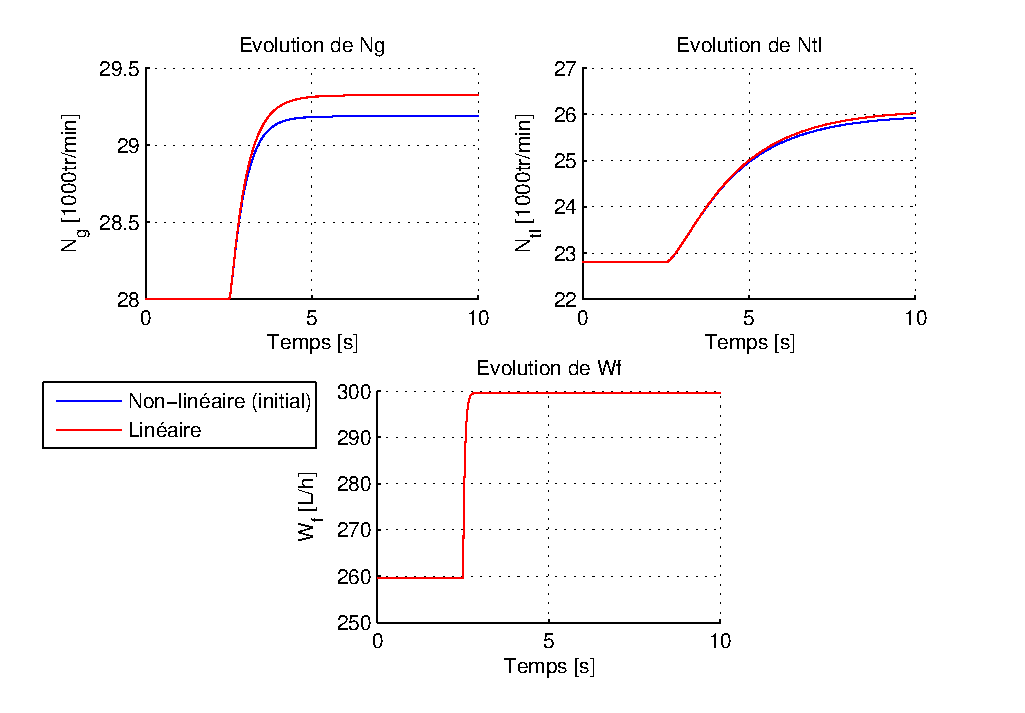
\includegraphics[scale=.9]{./figures/complet_vs_lin.eps}
\caption{Comparaison des performances entre le syst�me initial (non-lin�aire) et le syst�me lin�aris�}
\label{fig:complet_vs_lineaire}
\end{figure}

	

				
				

	\clearpage{}
	
	% !TEX encoding = IsoLatin
% --------------------------------------------------------------------------------------------------------------------------------------------------------------------------- %
%TODO : Figures EPS format for 3D matlab.......

\rhead{\footnotesize\rightmark}
\chapter{Observateur du Kalman}

\paragraph{}L'objectif du filtre de Kalman est d'estimer les �tats x(t) du syst�me � partir d'une s�rie de mesures incompl�tes ou bruit�es. Cet estim� not� $\hat{x}(t)$, est la sortie du filtre de Kalman. Ce filtre sugg�re une relation entr�es-sorties avec une optimisation des mesures. Le mod�le d'�tat de Kalman prend en compte les bruits d'entr�e (mod�le) et les bruits des capteurs de mesure des sorties. La notation propre au Kalman d'un mod�le avec bruit :

\begin{displaymath}
\begin{array}{l} \dot{x} \quad = \quad A.x(t) \quad + \quad B.u(t) + \quad M.w(t)\\ \\
y \quad = \quad C.x(t) \quad + \quad D.u(t) + \quad v(t) \end{array}
\end{displaymath}

\paragraph{}Certains hypotheses doivent �tre respect�es pour que la th�orie du filtre Kalman soit valable:\\

\begin{itemize}
\item [-] Le syst�me et les bruits sont stationnaires (Les matrices du mod�le d'�tat sont ind�pendantes du temps)
\item [-] La paire (A,C) est d�tectable, c'est � dire qu'il n'y a pas de mode instable et non observable dans le syst�me 
\item [-] Les signaux w(t) et v(t) sont des bruits blancs gaussiens centr�s.
\end{itemize}

\paragraph{}L'objectif dans cette partie est de filtrer les mesures des capteurs $N_g$, $N_{tl}$ et surtout offrir un estim� du d�bit r�el de carburant $W_f$. Pour cela nous r�alisons un estimateur/filtre de Kalman.

\paragraph{Remarque:}
\paragraph{}Le filtre de Kalman �tait sujet de TP pendant deux s�ances dans ce Bureau d'�tude. Les exercices faites nous ont permis d'approfondir les connaissances dans le principe et l'application du filtre de Kalman. 
		
	
	\section{�quations du filtre de Kalman}
	\paragraph{}Nous reprenons le mod�le lin�aris� pr�sent� � la fin du chapitre Lin�arisation. Nous supposerons donc que notre syst�me perturb� peut �tre mod�lis� par le mod�le d'�tat de Kalman parce qu'il satisfait les hypoth�ses n�cessaires. Nous avons utilis� les fonctions de Kalman propos� par le Toolbox Matlab parce que la solution obtenue est optimale. 
	
	\paragraph{}Le mod�le pris en compte pour calculer l'observateur de Kalman est le suivant :
		
\begin{displaymath}
\left\{ \begin{array}{l} \dot{x} \quad = \quad \left[ \begin{array}{cccc}
    -18.5185   &      0       &  0 \\
   65.5871 &  -1.9835   &      0 \\
   17.1650  &  0.8011  & -0.5289

\end{array}\right]  x \quad + \quad \left[ \begin{array}{cc}
 18.5185\\
         0 \\
         0 
\end{array} \right] u\\ \\
y \quad = \quad \left[ \begin{array}{cccc}
         0   & 1.0000     &    0 \\
    0.0020  &  0.0002    &     0 \\
    1.6012  & -0.0228    &     0 \\
         0  &       0   & 1.0000
\end{array} \right] x \quad + \quad \left[ \begin{array}{cc}
0\\
0\\
0\\
0
\end{array} \right] u \end{array}\right.
\end{displaymath}\\

\paragraph{}L'objectif est d'estimer l'entr�e du d�bit r�el de carburant $W_f$. Pour cela on diminue le mod�le en prenant une seule entr�e. L'entr�e $C_{charge}$ sera considerer comme une perturbation par la suite. 

\subsection{Incertitudes sur les donn�es}
\paragraph{}Dans le cahier des charges les incertitudes relatives sont donn�es pour chaque sortie. L'incertitude relative pr�sente un nombre sans dimension qui caract�rise la pr�cision de la mesure. Ce nombre est le rapport entre l'incertitude et la valeur mesur�e de la sortie. Pour chaque sortie estim�e nous pr�senterons les intervalles de variation autour les valeurs nominales.\\ 

\begin{itemize}
\item [-] $ N_g = 0.1\%$
\item [-] $ P_3 = 2\%$
\item [-] $ N_{tl} = 0.1\%$
\item [-] $ T_{45} = 2\%$
\end{itemize}

\paragraph{}Sur la figure suivante on peut observer les quatre sorties avec le bruit associ�. Dans le script simulink nous avons ajout� un bruit  pour chaque sortie avec le block \emph{Band Limited White noise}. Les valeurs de la densit� spectrale sont obtenues avec un produit de la pr�cision relative et une constante. La pr�cision relative nous donne la valeur de l'intervalle pour la sortie. Pour $N_{tl}$ la valeur nominale est $28000$, dont l'intervalle des valeurs est : $[28000 +\Delta N_g , 28000 -\Delta N_g ]$, avec $\Delta N_g = Precision * 28000$. 

	\begin{figure}[H]
\centering
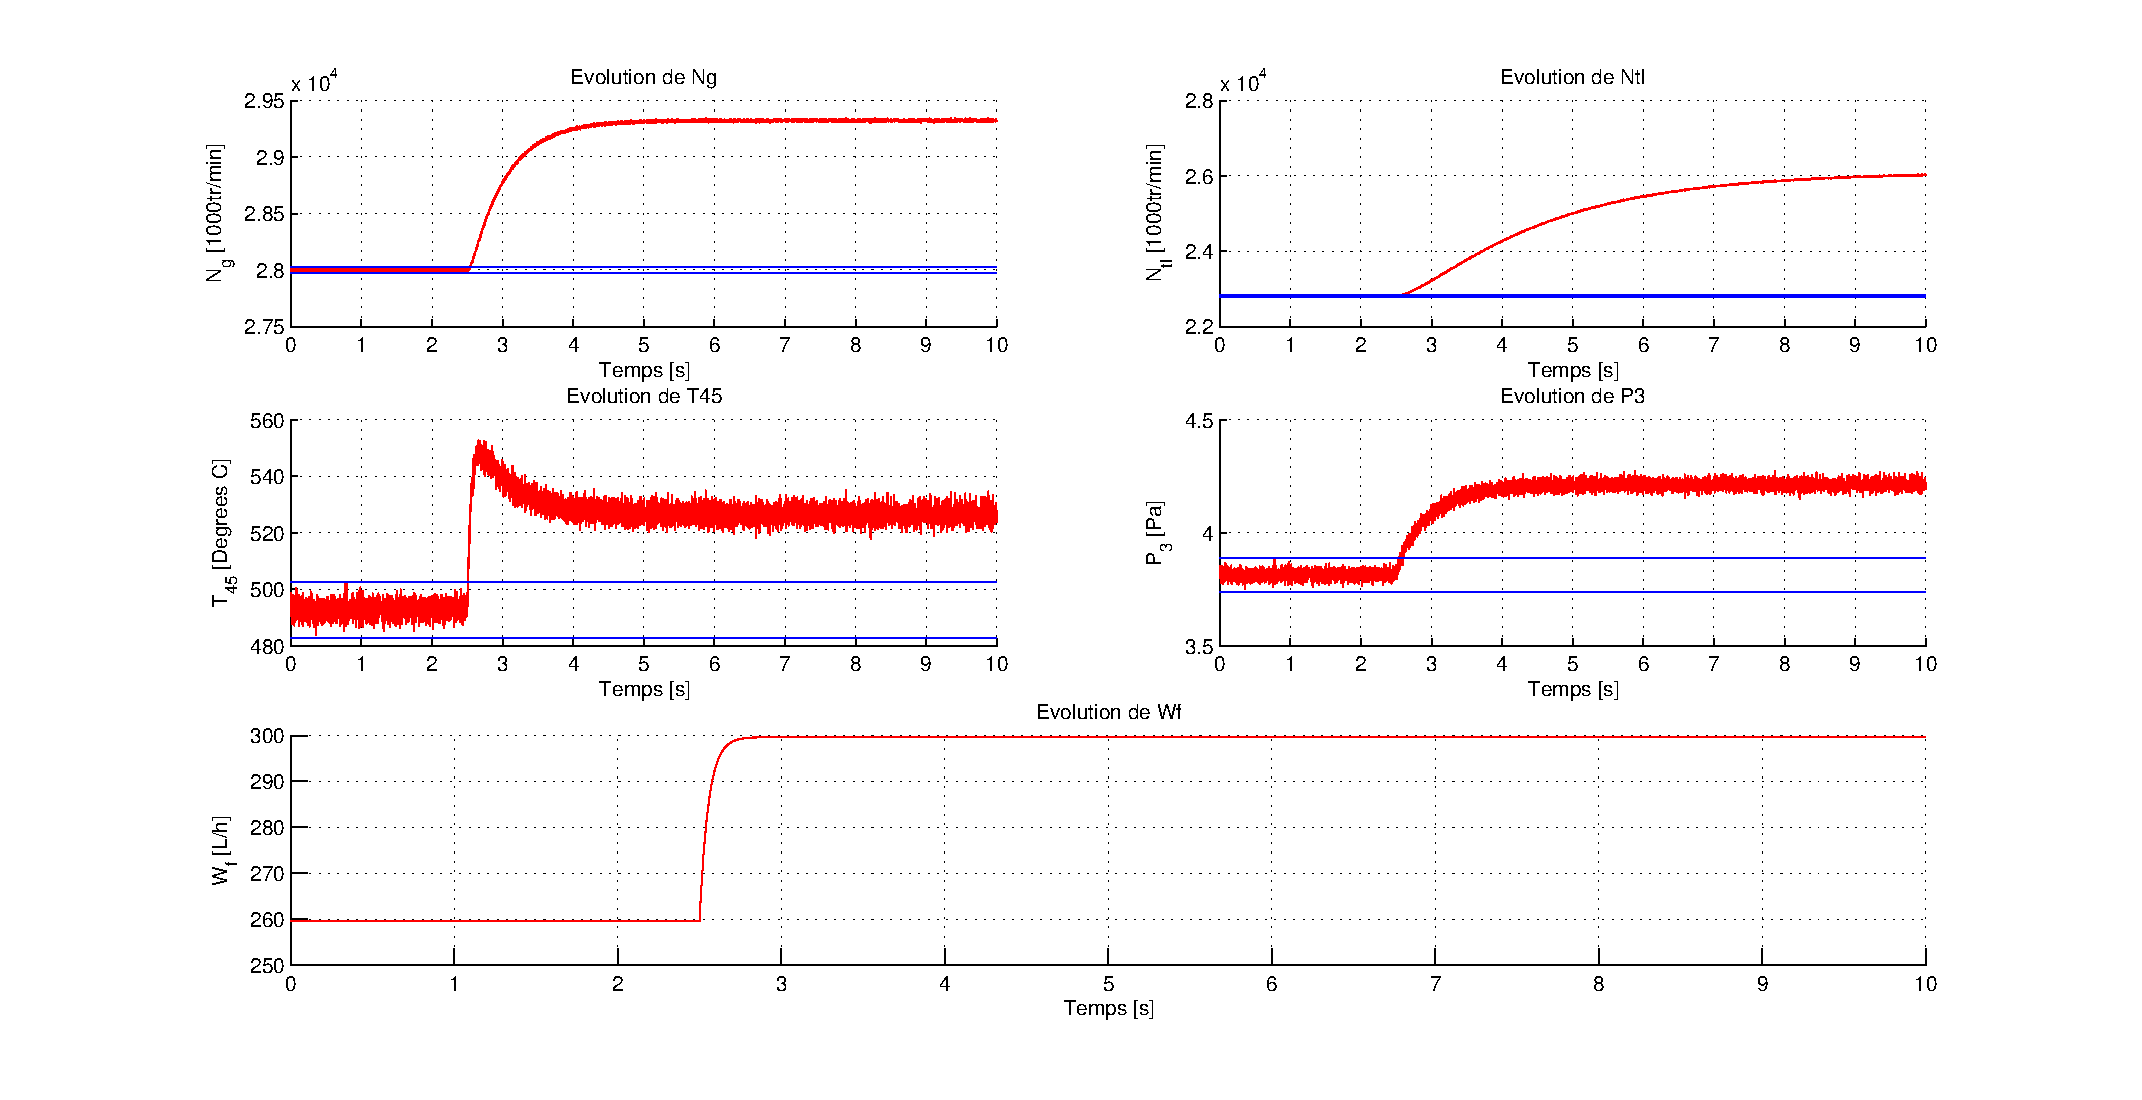
\includegraphics[scale=.45]{./figures/sortie_bruit.eps}
\caption{Signaux bruit�s de sortie en entr�e de l'observateur de Kalman}
\label{fig:sortie_bruit}
\end{figure}

\paragraph{}Dans le syst�me nous consid�rons que les bruits du mod�le ne sont par tr�s importants ($10^{-5}$). Les bruits de mesure sont importants ($10^{-3}$), autrement dit peu de confiance dans les capteurs. Les matrices suivantes pr�sentent la confiance dans les mesures (capteurs) et la confiance dans le mod�le respectivement (matrices de covariance) :
\begin{equation}		
R_{N} =
 \begin{pmatrix}
  0.001 & 0 & 0 & 0\\
  0 & 0.001 & 0 & 0\\
  0 & 0 & 0.001 & 0\\
  0 & 0 & 0 & 0.001
 \end{pmatrix}
\quad et
\quad Q_{N} =
 \begin{pmatrix}
  0.00001 
  \end{pmatrix}
\end{equation}

\paragraph{}Les termes sur la diagonale de la matrice $R_N$ correspond au carr� des �cart-types maximaux de l'erreur que l'on autorise pour chacun des param�tres � estimer. Les valeurs choisies correspondent � l'estimation sur les sorties et la valeur d'erreur autoris�e. Il faut avoir conscience que si on d�finie des termes d'erreur trop petit par rapport � la r�alit�, le filtre de Kalman n'arrivera pas � rectifier les erreurs du mod�le et fera des estimations biais�s. Si les erreurs sont trop importantes par rapport � la r�alit�, les estimations seront avec une covariance importante. Pour avoir la meilleure estimation nous avons choisi la m�me variance sur chaque param�tre en respectant les pr�cision r�elles des capteurs. 
	
	\section{Calcul du gain de Kalman}
	\paragraph{}Avec la commande kalman sous \emph{Matlab} on obtient le gain du filtre et aussi la solution de l'�quation de Ricatti qui donne la matrice de covariance de l'estimation d'erreur. Ensuite on simplifie le mod�le d'�tat et on garde que les entr�es et les sorties du observateur qui sont demand�es dans le cahier des charges. La formule utilis�e pour calculer le mod�le d'�tat est :
	
	\begin{equation}
	A_{kalman} = A_{lin} - K.C_{lin} \quad
	B_{kalman} = [B_{lin}\quad K] \quad
	C_{kalman} = I_{3} \quad
	D_{kalman} = 0_{3}
	\end{equation}
	
	Le mod�le obtenu du filtre de Kalman est : 

	\begin{displaymath}
\left\{ \begin{array}{l} \dot{x} \quad = \quad \left[ \begin{array}{cccc}
-18.74 &  -0.2354 & -0.06749\\
 65.11  &  -5.711  &  -1.564\\
 17.05 &  -0.7616  &  -1.628
\end{array}\right]  x \quad + \quad \left[ \begin{array}{ccccc}
18.52 & 0.2386 & 0.0002408 & 0.1393 & 0.06749\\
0 & 3.735 & 0.001385 & 0.297 & 1.564\\
0 & 1.564 & 0.0005146 & 0.07243 & 1.099
\end{array} \right] u\\ \\
y \quad = \quad \left[ \begin{array}{ccc}
         1 & 0  & 0 \\
    0 & 1 & 0 \\
         0 & 0 & 1
\end{array} \right] x \quad + \quad \left[ \begin{array}{ccccc}
         0 & 0 & 0 & 0     &    0 \\
    0 & 0 & 0 & 0 & 0\\
         0 & 0 & 0 & 0 & 0
\end{array} \right] u \end{array}\right.
\end{displaymath}\\
	
\paragraph{}Ce mod�le prend en entr�e toutes les sorties du syst�me lin�aire et le d�bit du carburant $W_f$. En sortie du filtre de Kalman il donne les trois estimations : $W_f$, $N_g$ et $N_{tl}$ (les trois �tats du syst�me). La figure suivante montre l'estimation du filtre de Kalman sur le vecteur d'�tat. L'allure des r�ponses correspond � une �volution suite � un changement de la consigne $W_f$. Le filtre de Kalman estime bien ses sorties : $W_f$, $N_{g}$ et $N_{tl}$.

% Insert figure kalman estimation

	\begin{figure}[H]
\centering
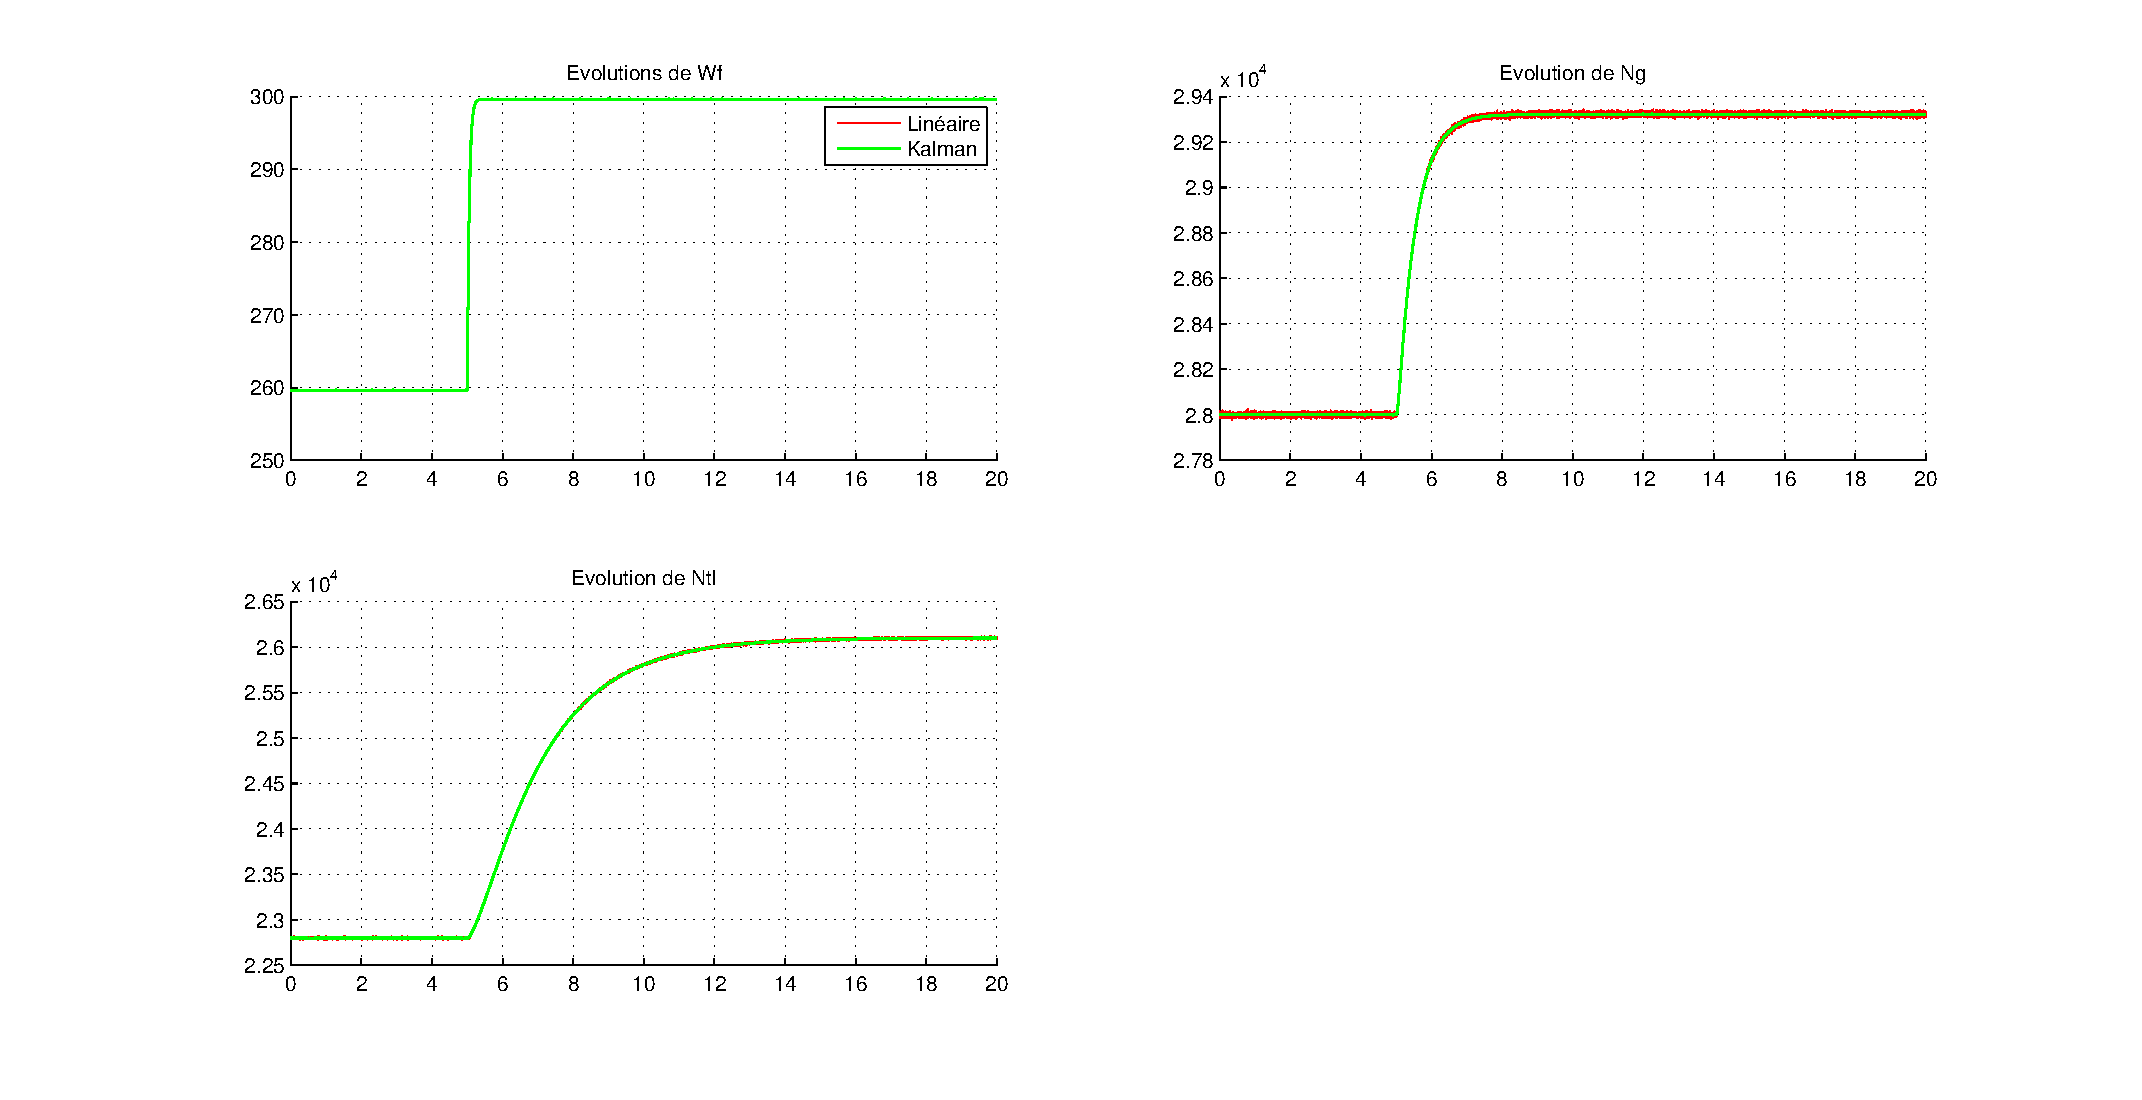
\includegraphics[scale=.45]{./figures/resultat_kalman.eps}
\caption{Signaux bruit�s et filtr�s en sortie de l'observateur de Kalman}
\label{fig:resultat_kalman}
\end{figure}

% Futur propositions et �volutions (Observateur a gain variable)	
\paragraph{Observateur � gain variable}
\paragraph{}L'int�r�t d'utiliser un observateur � gain variable est d'estimer un syst�me non lin�aire. Autrement dit on doit appliquer un filtre de Kalman �tendu. Ce filtre permet en effet de lin�ariser localement le probl�me et donc d'appliquer les �quations du filtre de Kalman classique. Parce qu'on doit localiser le syst�me autour d'un point d'�quilibre � chaque �tape, ceci assure donc la convergence locale de l'erreur, mais non celle globale. Un surco�t de calcul est constat� par rapport au filtre de Kalman classique. En effet, outre les op�rations non lin�aires introduit dans les �quations d'�tats et de transitions, il faut recalculer � chaque �tape les Jacobiennes de ces �quations.

\paragraph{}Une autre avantage du gain variable est pour cr�er des r�sidus afin de d�tecter les pannes des capteurs. En appliquant un gain variable la dynamique du mod�le change, et il peut perdre la stabilit� asymptotique.


	\clearpage{}
	
	% !TEX encoding = IsoLatin
% --------------------------------------------------------------------------------------------------------------------------------------------------------------------------- %
%\begin{itemize}
%\item [-] \textbf{Cr�ation} : Demand�e par un autre processus,  cr�e dans l'�tat pr�t ou suspendu.
%\item [-] \textbf{Destruction} : peut �tre fait par le processus lui-m�me, un autre processus, le noyau. La destruction provoque une lib�ration des ressources associ�es et un �v�nement.
%\item [-] \textbf{Blocage} : passage en mode bloqu� en attente d'un �v�nement externe. Peut �tre demand� par le processus lui-m�me ou par le syst�me.
%\item [-] \textbf{D�blocage} : passage en mode pr�t apr�s le mode bloqu� lorsque l'�v�nement attendu se produit.
%\item [-] \textbf{Activation} : passage en mode ex�cution d'un mode pr�t.
%\end{itemize}

  
%\begin{Verbatim}[frame=single,fontsize=\scriptsize]
%\end{Verbatim}

%\begin{figure}[h]
%	\begin{center}
%		\includegraphics[width=14.5cm,height=9cm]{.\figures\diag_etat_threads.png}
%	\end{center}
%	\caption{Diagramme des diff�rents �tats d'un thread avec les primitives}
%	\label{fig:diag_etat_threads}
%\end{figure}

%% Modele d'etat avec les matrices

%\begin{displaymath}
%\left\{ \begin{array}{l} \dot{x} \quad = \quad \left[ \begin{array}{cccc}
%0 & 1 & 0 & 1\\
%- \frac{K_s}{M_s} & - \frac{C_s}{M_s} & 0 & \frac{C_s}{M_s}\\
%0 & 0 & 0 & 1\\
%\frac{K_s}{M_u} & \frac{C_s}{M_u} & - \frac{K_t}{M_u} & - \frac{C_s}{M_u} - \frac{C_t}{M_u}
%
%\end{array}\right]  x \quad + \quad \left[ \begin{array}{cc}
%0 & 1.1972\\
%0 & - 0.0012\\
%0 & 0\\
%7.84 & - 4.05
%\end{array} \right] u\\ \\
%y \quad = \quad \left[ \begin{array}{cccc}
%1 & 0 & 0 & 0\\
%0 & \lambda & 0 & 0\\
%0 & 0 & \lambda & 0\\
%0 & 0 & 0 & \lambda\\
%0 & - \lambda & \lambda & 0
%\end{array} \right] x \quad + \quad \left[ \begin{array}{cc}
%0 & 0\\
%0 & 0\\
%0 & 0\\
%0 & 0\\
%0 & 0
%\end{array} \right] u \end{array}\right.
%\end{displaymath}\\

% --------------------------------------------------------------------------------------------------------------------------------------------------------------------------- %
\rhead{\footnotesize\rightmark}
\chapter{Commande par retour d'�tat}
L'objectif de cette partie est de concevoir une commande par retour d'�tat qui respecte certains contraintes en prenant directement l'�tat mesur� sur le mod�le lin�arit� non bruit�. La commande doit imposer une simple r�gulation de la turbine autour d'un point de fonctionnement. L'hypoth�se est que le syst�me est commandable et observable. La conception de cette commande permet de placer les p�les du syst�me en boucle ferm�e. En fonction du cahier des charges (temps de r�ponse, d�passement, bande passante) on va placer les p�les afin d'avoir un syst�me asymptotiquement stable et qui respecte les performances souhait�es. 

	\section{Performances du syst�me lin�aris�}
	\paragraph{}Avant d'appliquer la commande par retour d'�tat il faut v�rifier les performances du syst�me lin�aris�. La premi�re propri�t� est la stabilit�. Les valeurs propres sont toutes � partie r�elle n�gative, donc le syst�me est asymptotiquement stable. Les valeurs propres de la matrice dynamique $A_{lin}$ sont : 
	\begin{equation}
	\lambda_1 = -0.5289 \quad \lambda_2 = -1.9835 \quad \lambda_3 = -18.5185 
	\end{equation}
	
	\paragraph{}Si on trace les r�ponses impulsionnelles du syst�me lin�aris� on peut remarquer que certains sorties ne d�pendent que d'une entr�e. $N_{tl}$ ne d�pend que de $C_{charge}$ et les autres d�pendent que de $W_f$. Le temps de r�ponse est inf�rieur � 5s et le d�passement est n�gligeable. L'objectif de notre commande par retour d'�tat sera de respecter le cahier des charges et de ne pas trop modifier le fonctionnement nominal du syst�me.
	
	\section{Cahier des charges}
	\paragraph{}La loi de commande doit assurer un asservissement de la vitesse de la turbine libre $N_{tl}$ autour de sa valeur nominale. L'erreur statique doit �tre nulle malgr� les variations de la charge utile $C_{charge}$, que nous consid�rons comme une r�elle perturbation. La stabilit� du syst�me sera d�montr�e et la dynamique sera optimis�e par la suite. 
	
	\paragraph{}Le correcteur de retour d'�tat doit respecter les contraintes suivantes :\\
\begin{itemize}
\item [-] Erreur statique sur $N_{tl}$ nulle sur toute la plage
\item [-] Respecter les capacit�s de la turbine : d�bit wf ne d�passant pas excessivement la limite du slew rate et le d�bit maximal
\item [-] Marge de phase de 60 degr�s
\item [-] Protection de la turbine : D�bit minimal $W_f^{min}$ = $60 \frac{l}{h}$
\item [-] D�bit de carburant maximum $W_f^{max}(P3)$
\item [-] Slew rate $\dot{W_f}_{max}$ = $100 \frac{l/h}{s}$ 
\end{itemize}

	\paragraph{}Ces contraintes doivent �tre respect�es quand le pire �chelon sera appliquer dans le syst�me.
		
	\section{Placement de p�les}
	L'id�e de placement de p�les est de simplifier la dynamique du syst�me lin�aris� en une dynamique d'un syst�me de second ordre. On peut facilement calculer les p�les en fonction du temps de r�ponse et du d�passement souhait�. En partant de la fonction du transfert d'un syst�me du second ordre :
	\begin{equation}
	G = \frac{K.\omega_{n}^2}{s^2 + 2.\zeta.\omega_n + \omega_{n}^2}	
	\end{equation}

	d'o� les deux p�les en fonction de coefficient d'amortissement $\zeta$ et de la pulsation propre $\omega_n$:
	\begin{equation}
	[p1;p2] = -\zeta.\omega_n \pm i.\omega_n.\sqrt{1-\zeta^2}
	\end{equation}

	\paragraph{}L'objectif est de limiter le d�passement de la r�ponse impulsionnelle dans le cas d'un pire �chelon de charge. On impose un d�passement inf�rieur � 5\%. Cela veut dire que le coefficient d'amortissement doit �tre sup�rieur � $\frac{\sqrt{2}}{2}$. La pulsation propre $\omega_n$ est calcul�e avec la formule :
	\begin{equation}
	-\zeta.\omega_n \leq -\frac{4.5}{t_r}
	\end{equation}

	\paragraph{}Les valeurs obtenues pour les poles sont:
	\begin{equation}
	[p1;p2] = -4.5000 \pm i.3.9411\quad
	p3 = -5
	\end{equation}
\paragraph{}Le troisi�me p�le est r�el n�gatif et plus rapide que les deux p�les conjugu�s. Autrement dit les premiers deux p�les seront dominants et satisferont la performance du r�gime transitoire du syst�me demand�e dans le cahier des charges. Cette m�thode permet de r�gler la dynamique du syst�me en r�gime transitoire. On remarque que plus les p�les sont n�gatifs (rapides) plus le syst�me consomme d'�nergie afin d'�tablir la commande. Si le temps de r�ponse diminue, l'�nergie consomm�e par la commande diminue. 
	
	\paragraph{}L'objectif de la commande est d'avoir une erreur statique nulle qui ne d�pend pas de la perturbation $C_{charge}$. Avec ces trois p�les la commande ne peut jamais satisfaire cette contrainte. Pour avoir une erreur statique nulle il faut ajouter un int�grateur dans le mod�le d'�tat. Pour cela on va changer le mod�le d'�tat.
	
	\section{Retour d'�tat augment�}
	Pour mieux satisfaire la contrainte d'erreur statique nulle on ajoute l'int�grateur dans le mod�le d'�tat. De cette fa�on on peut r�utiliser ce mod�le d'�tat pour l'observateur de Kalman. Si on ajoute un int�grateur en dehors du syst�me il faut pr�voir plusieurs calculs pour r�pondre aux m�mes contraintes. 
	
	\paragraph{}On va ajouter un �tat suppl�mentaire dans la matrice dynamique qui est l'int�grale de $N_{tl}$. le mod�le devient :
		\begin{displaymath}
\left\{ \begin{array}{l} \dot{x} \quad = \quad \left[ \begin{array}{cccc}

  -18.5185     &    0     &    0      &   0\\
   65.5871 &   -1.9835  &       0   &      0\\
   17.1650  &  0.8011 &  -0.5289   &      0\\
         0   &      0  &  1.0000    &     0
\end{array}\right]  x \quad + \quad \left[ \begin{array}{ccccc}
   18.5185      &   0\\
         0     &    0\\
         0 & -381.2529\\
         0   &      0
\end{array} \right] u\\ \\
y \quad = \quad \left[ \begin{array}{ccccc}
         0   & 1.0000        & 0   &      0\\
    0.0020  &  0.0002   &      0    &     0\\
    1.6012 &  -0.0228   &      0    &     0\\
         0   &      0  &  1.0000    &     0\\
         0    &     0    &     0   & 1.0000
\end{array} \right] x \quad + \quad \left[ \begin{array}{ccccc}
         0 & 0  \\
    	0 & 0  \\
	0 & 0  \\
	0 & 0  \\
	0 & 0 
\end{array} \right] u \end{array}\right.
\end{displaymath}\\
	
	\paragraph{}Pour le placement de p�le maintenant nous avons quatre p�les � placer. Nous allons utiliser la m�me m�thode que pr�c�demment. Les premiers deux p�les seront ceux qui fixent le r�gime transitoire. Les deux autres seront plac�s tr�s loin avec un temps de r�ponse plus rapide. Les valeurs sont : 
	\begin{equation}
	[p1;p2] = -0.2250 \pm i.0.2069\quad
	p3 = -11.25 \quad
	p4 = -9
	\end{equation}
	
	Le gain du retour d'�tat est : 
	\begin{equation}
		K = \begin{pmatrix}
   -0.0179  &  0.0538 &  -0.0050  &  0.0059
		\end{pmatrix}
	\end{equation}	
	
	\paragraph{}Avant de faire la simulation nous ajoutons les saturateurs dans le sch�ma Simulink (cf. \ref{fig:simulink_retour_etat_aug}). On peut observer les variations de la r�ponse impulsionnelle de $N_{tl}$ quand la consigne de la charge change de valeur. En r�gime statique l'erreur statique reste nulle. Le r�gime transitoire ne correspond pas aux performances souhait�es. Nous remarquons un d�passement assez important et en temps de r�ponse lent. L'objectif est de respecter la variation de la commande. �a permet d'optimiser l'�nergie consomm�e par la commande. 
	
	TODO : figure de Mod�le augment�. (Julien)
	
	\paragraph{}Si on diminue le temps de r�ponse le d�passement diminue �galement. Autre moyen est de changer les saturateurs et augmenter les limites de variation. Pour respecter le cahier des charges nous devons faire une commande $H_\infty$. Cela optimise la commande en respectant son �nergie.  
	
	TODO : explication de la courbe et �volution du r�gime transitoire en fonction de placement des p�les. 
	
	\section{Pire �chelon de charge}
	\paragraph{}Le pire �chelon est d�fini par un �chelon qui va de la charge minimale � la charge maximale (�quilibr� autour de $(W_f)_{min}$ et $(W_f)_{max}=isowf(end)$). La rapidit� maximale est limit�e � $64m.\frac{daN}{s}$. Les valeurs obtenues sont :\\
	
\begin{itemize}
\item [-] $Wf_{min}$ = -199.6451
\item [-] $Wf_min$ = 38.3780
\item [-] $(C_{charge})_{min}$ = -10.3398
\item [-] $(C_{charge})_{max}$ = 1.6522
\end{itemize}		
	\clearpage{}
	
	% !TEX encoding = IsoLatin
% --------------------------------------------------------------------------------------------------------------------------------------------------------------------------- %
%\begin{itemize}
%\item [-] \textbf{Cr�ation} : Demand�e par un autre processus,  cr�e dans l'�tat pr�t ou suspendu.
%\item [-] \textbf{Destruction} : peut �tre fait par le processus lui-m�me, un autre processus, le noyau. La destruction provoque une lib�ration des ressources associ�es et un �v�nement.
%\item [-] \textbf{Blocage} : passage en mode bloqu� en attente d'un �v�nement externe. Peut �tre demand� par le processus lui-m�me ou par le syst�me.
%\item [-] \textbf{D�blocage} : passage en mode pr�t apr�s le mode bloqu� lorsque l'�v�nement attendu se produit.
%\item [-] \textbf{Activation} : passage en mode ex�cution d'un mode pr�t.
%\end{itemize}

  
%\begin{Verbatim}[frame=single,fontsize=\scriptsize]
%\end{Verbatim}

%\begin{figure}[h]
%	\begin{center}
%		\includegraphics[width=14.5cm,height=9cm]{.\figures\diag_etat_threads.png}
%	\end{center}
%	\caption{Diagramme des diff�rents �tats d'un thread avec les primitives}
%	\label{fig:diag_etat_threads}
%\end{figure}

%% Modele d'etat avec les matrices

%\begin{displaymath}
%\left\{ \begin{array}{l} \dot{x} \quad = \quad \left[ \begin{array}{cccc}
%0 & 1 & 0 & 1\\
%- \frac{K_s}{M_s} & - \frac{C_s}{M_s} & 0 & \frac{C_s}{M_s}\\
%0 & 0 & 0 & 1\\
%\frac{K_s}{M_u} & \frac{C_s}{M_u} & - \frac{K_t}{M_u} & - \frac{C_s}{M_u} - \frac{C_t}{M_u}
%
%\end{array}\right]  x \quad + \quad \left[ \begin{array}{cc}
%0 & 1.1972\\
%0 & - 0.0012\\
%0 & 0\\
%7.84 & - 4.05
%\end{array} \right] u\\ \\
%y \quad = \quad \left[ \begin{array}{cccc}
%1 & 0 & 0 & 0\\
%0 & \lambda & 0 & 0\\
%0 & 0 & \lambda & 0\\
%0 & 0 & 0 & \lambda\\
%0 & - \lambda & \lambda & 0
%\end{array} \right] x \quad + \quad \left[ \begin{array}{cc}
%0 & 0\\
%0 & 0\\
%0 & 0\\
%0 & 0\\
%0 & 0
%\end{array} \right] u \end{array}\right.
%\end{displaymath}\\

% --------------------------------------------------------------------------------------------------------------------------------------------------------------------------- %
\rhead{\footnotesize\rightmark}
\chapter{Commande robuste}

\textcolor{red}{Maffre}

	Un retour d'�tat $K$ stabilisant le syst�me et rejetant, au mieux, les perturbations (couple r�sistant $C_{charge}$) ayant �t� calcul� pour le point de fonctionnement ($X_0$, $U_0$) consid�r�, il est maintenant n�cessaire de v�rifier la stabilit� du syst�me boucl� pour des points de fonctionnement diff�rents. En effet, le point d'�quilibre peut �tre en r�alit� l�g�rement diff�rent ce celui calcul� dans le chapitre 2. \\
	
	Nous utiliserons pour cela des m�thodes de calcul \textit{LMI} (Linear Matrix Inequalities) (toolbox \texttt{lmi} de Matlab).


	\section{Calcul du retour d'�tat $K_{lmi}$ stabilisant}
	
		Nous allons tout d'abord recalculer un gain de retour d'�tat stabilisant le syst�me (not� $K_{lmi}$). Cet exercice est bien entendu redondant par rapport � la partie pr�c�dente mais il permet d'introduire les \textit{LMI}. \\
		
		La th�orie des \textit{LMI} que l'existence d'une matrice sym�trique $P$ satisfaisant la th�orie de Lyapunov est une condition n�cessaire et suffisante de stabilit� pouvant �tre d�crite par l'�quation : 
		
		\begin{align}
			PA^T + AP & < 0 \\
			P & > 0 
		\end{align}
		
		La matrice dynamique $A$ d'un syst�me boucl� avec un gain de retour d'�tat $u = -Kx$ �tant �gale � $A_{boucl�} = (A - BK)$, on aura alors la \textit{LMI} suivante comme condition n�cessaire et suffisante de stabilit� : 
		
		\begin{align}
			P(A-BK)^T + (A+BK)P & < 0 \\
			P & > 0 
		\end{align}
		
		Cette \textit{LMI} �tant non-lin�aire, il est n�cessaire d'effectuer le changement de variable $K = LP^{-1}$ pour assurer sa lin�arit�.
		
		\begin{align}
			PA^T + AP + L^TB + BL & < 0  \\
			P & > 0 
		\end{align}
		
		La matrice $K_{lmi}$ retourn�e par le script Matlab est alors telle que : 
		
		\begin{equation}
			K_{lmi} = [1.0042   -4.0059   -2.3667   -1.9401]
		\end{equation}
		
		Et permet d'assurer la stabilit� du syst�me en pla�ant les p�les dans le demi-plan gauche du plan complexe. Cependant, comme aucune autre sp�cification sur le placement des p�les n'est donn�e, le solveur \textit{LMI} se contente de trouver un seul gain qui stabilise le syst�me. Autrement dit, la derni�re it�ration correspond � l'it�ration � laquelle le solveur a trouv� pour la premi�re fois un gain stabilisant. \\ 
		
		L'objectif est maintenant de sp�cifier des r�gions \textit{LMI} (� l'aide par exemple de la commande \texttt{lmireg})pour que les p�les en boucle ferm�e appartiennent � l'intersection de ces r�gions. Ces r�gions correspondent � : 
		
		\begin{itemize}
			\item Un demi-plan dont la partie r�elle est inf�rieure � une valeur n�gative $x_0$ donn�e, sp�cifiant alors le \textbf{temps de r�ponse du syst�me}.
			\item Un demi-plan dont la partie r�elle est sup�rieure � une valeur n�gative $x_1$ (telle que $x_1 < x_0$) donn�e, pour \textbf{rester dans la bande passante} du syst�me.
			\item Un secteur conique dont la pointe est situ�e � l'origine du plan complexe, pour fixer l'amortissement et donc \textbf{limiter le d�passement}.
		\end{itemize}
		
		
		
		
		
		
		
		
	
	
	
	\section{V�rification de la stabilit� du syst�me}

	\clearpage{}
	
	\chapter*{Conclusion}
	\addcontentsline{toc}{chapter}{Conclusion}
	% !TEX encoding = IsoLatin
\paragraph{OBJECTIF}
\paragraph{}Durant ce bureau d'�tude nous avons mis en application diff�rentes notions vues en cours d'automatique avanc�e afin de commander une turbine � gaz. L'objectif est de suivre une d�marche industrielle de conception d'un syst�me de commande. 

\paragraph{BILAN}
\paragraph{}Tout d'abord nous avons mod�lis� la turbine � l'aide des �quations fondamentales de la m�canique. 


\paragraph{FUTUR}
\paragraph{}Ce bureau d'�tude nous a donc permis de mettre en place sur un cas concret deux commandes fondamentales de l'automatique, de nous rendre compte des difficult�s qu'elles impliquent (notamment au niveau du calcul des param�tres) mais aussi de leur efficacit� et de leur grande utilit�.
\paragraph{}Le sujet choisi pour mettre en oeuvre ce bureau d'�tude est tr�s parlant et a le m�rite d'�tre complet.

	\clearpage{}
	
	
	\listoffigures 	
	
	%\input{biblio}
	\clearpage{}
	
%\definecolor{listinggray}{gray}{0.9}
%\definecolor{lbcolor}{rgb}{0.9,0.9,0.9}
%
%\definecolor{colKeys}{rgb}{0,0,1} 
%\definecolor{colIdentifier}{rgb}{0,0,0} 
%\definecolor{colComments}{rgb}{0.1,0.5,0.1} 
%\definecolor{colString}{rgb}{0.6,0.1,0.1} 
%	
%	%% Annexe code MATLAB
%	\chapter*{Annexes}
%	
%\addcontentsline{toc}{chapter}{Annexes}
%\lstset{inputencoding=utf8/latin1,
%	tabsize=4,
%	rulecolor=,
%	language=MATLAB,
%        basicstyle=\scriptsize,
%        upquote=true,
%        aboveskip={1.5\baselineskip},
%        columns=fixed,
%        showstringspaces=false,
%        extendedchars=true,
%        breaklines=true,
%        prebreak = \raisebox{0ex}[0ex][0ex]{\ensuremath{\hookleftarrow}},
%        frame=single,
%        showtabs=false,
%        showspaces=false,
%        showstringspaces=false,
%        identifierstyle=\ttfamily,
%  identifierstyle=\color{colIdentifier}, 
%  keywordstyle=\color{colKeys},
%  stringstyle=\color{colString}, 
%  commentstyle=\color{colComments}} 
%\renewcommand{\thesection}{\Alph{section}}
%\setcounter{section}{0}
%\section{script\_MATLAB.m}
%\label{annexe}
%\lstinputlisting{script_MATLAB.m}
	
\label{pagefin}

\end{document}